\documentclass[zihao=-4,a4paper,fontset=none]{ctexart}
\usepackage[a4paper,margin=2.5cm]{geometry}
\usepackage{amsmath,amssymb}
\usepackage{graphicx}
\usepackage{booktabs}
\usepackage{setspace}
\usepackage{indentfirst}
\usepackage[font=small]{caption}
\graphicspath{{figs/}}

% 中文字体（系统 Noto CJK）
\setCJKmainfont[BoldFont={Noto Serif CJK SC Bold}]{Noto Serif CJK SC}
\setCJKsansfont{Noto Sans CJK SC}
\setCJKmonofont{Noto Sans Mono CJK SC}

\setstretch{1.25}
\ctexset{
  section={beforeskip=0.9em,afterskip=0.5em},
  subsection={beforeskip=0.6em,afterskip=0.4em}
}
\allowdisplaybreaks

\begin{document}

% ===================== 标题与摘要 =====================
\begin{center}
{\zihao{3}\bfseries 基于线性规划与对偶分析的微网计划购电策略}
\end{center}

\vspace{0.3em}
\centerline{\textbf{摘\quad 要}}
% TODO 摘要：各问完成后撰写（deAiWriting 摘要三段式）：
% ① 问题锚定：微网光-储-负荷协同、双谷双峰分时电价；② 分问题链路（每问"数据→模型→
% 算法→数值结论"）；③ 验证与特色（三重校验、阈值 1/0.81、规则式对照 +11.71%）
（占位）摘要待问题 2--4 完成后统一撰写。本问已备妥的数值结论：全天购电 59482.7 kWh、购电费 35126.85 元，较无储能运行节省 26.9\%；充放电启停受阈值 $1/0.81\approx1.235$ 支配；规则式策略较线性规划最优贵 11.71\%。

\vspace{0.2em}
\centerline{\textbf{关键词：}\ 微网；分时电价；储能调度；线性规划；对偶分析}

% ===================== 1 问题重述 =====================
\section{问题重述}
% TODO（骨架）：一段背景（微网消纳分布式光伏、外网分时电价、储能低充高放）；
% 一段逐问概述：P1 每天电价负载相同+光伏预测，0:00 制定计划购电策略（供电不低于负载、
% 储能 0:00 与 24:00 同电量），输出表 1/表 2 与 result1.xlsx；P2 实际数据+5 倍紧急购电；
% P3 0/6/12/18 点滚动预报与调整购电（0.5 倍违约、1.5 倍超购）；P4 波动电价重算 P2/P3。

% ===================== 2 问题分析 =====================
\section{问题分析}
% TODO（骨架）：P1 完全信息确定性场景→线性规划可证精确最优（对比 DP 离散化与规则式）；
% 逐问分析思路各一句，问题 2/3/4 完成后补齐。

% ===================== 3 模型假设 =====================
\section{模型假设}

\begin{enumerate}
\item \textbf{日周期性}：附件~1 的电价与负载曲线逐日相同，光伏预测为同一日曲线（电价 0.3713~1.3952 元/kWh、负载 3309~5959~kW、光伏 0~7612.3~kW），计划得以逐日复制，这是 5.1 节时段映射的依据。
\item \textbf{储能效率口径}：充、放电效率各取 $90\%$，往返效率 $81\%$，损耗只发生在进出储能的路径上，直供负载不打折。设计说明：题面只给"充放电效率为 $90\%$"一个数值，两种记法在文献中都有，文献~\cite{wangxz2017} 对充、放分别取 93\% 与 92\%，文献~\cite{sioshansi2009} 把往返效率记在充电侧；本文取前者，若改按"往返合计 $90\%$"重解，成本为 33416.43 元、低 4.87\%，差异不影响模型结构，声明口径即可。
\item \textbf{功率上限口径}：5000~kW 指储能设备并网侧，即母线端的充、放电功率，两个方向对称；计入效率后电池侧存入不超过 4500~kW、放出不超过 5556~kW，与表~\ref{tab:charge} 的母线计量一致。
\item \textbf{不售电}：购电量与放电量均非负，不向外网反送电；光伏盈余只能充电或弃掉，弃光不计费用，以与题面"购电量"的记账方向一致。
\item \textbf{完全信息}：0:00 制定计划时全天电价、负载与光伏预测已知且无误差，问题~1 为确定性规划，预测误差与缺电惩罚留给问题~2、3。
\end{enumerate}

% ===================== 4 符号说明 =====================
\section{符号说明}

{\small
\begin{center}
\begin{tabular}{ll}
\toprule
符号 & 说明 \\
\midrule
$\Delta t$ & 单时段长度，10 min，即 $1/6$ h \\
$\lambda_t$ & 时段 $t$ 的外网电价，元/kWh \\
$L_t$ & 时段 $t$ 的小区负载，kW \\
$P_t^{\mathrm{pv}}$ & 时段 $t$ 的光伏发电预测功率，kW \\
$a_t,\ b_t$ & 时段 $t$ 购电功率：直供负载 / 充电，kW \\
$g_t,\ c_t$ & 时段 $t$ 光伏功率：直供负载 / 充电，kW \\
$d_t,\ q_t$ & 时段 $t$ 储能放电功率，并网侧 / 弃光功率，kW \\
$E_t$ & 时段 $t$ 末储电量，kWh \\
$\eta$ & 充放电效率，取 0.9 \\
$E_0,\ E_{\min},\ E_{\max}$ & 储电量初值与界限：6000、1200、10800 kWh \\
$P_{\max}$ & 并网侧充放电功率上限，5000 kW \\
$\gamma_t,\ \sigma_t$ & 节点边际价值 / 边际供电成本，元/kWh \\
\bottomrule
\end{tabular}
\end{center}
}
其余局部符号在首次出现处说明。

% ===================== 5 问题1 =====================
\section{问题1模型的建立与求解}

\subsection{数据预处理}

附件~1 给出 144 行、间隔 10 分钟的电价、小区负载与光伏发电预测功率。电价在 0.3713~1.3952 元/kWh 之间，峰谷比约 3.76；负载 3309~5959~kW；光伏峰值 7612.3~kW，正出力区间约为 4:40 至 19:30。电价在深夜 23 时前后与午间 11 时至 13 时各有一个低谷，早 8 时前后与 19 时至 22 时各有一个高峰，双谷双峰的形态足以支撑储能低充高放。

各行的时间标签为时段起点，依次为 0:10、0:20、……、23:50 与 0:00+1。据此把当日划成 144 个日历时段 $I_k=[10(k-1),\,10k)$ 分钟，$k=1,\dots,144$：时段 $I_2$ 至 $I_{144}$ 依次取附件的第 1 至第 143 行，$I_1$ 取第 144 行，原因是该行标记的是次日 0:00 起的 10 分钟，由假设~1 的周期性，它与当日 0:00 至 0:10 的数据完全相同。结果模板要求填写 144 个购电量，标签自 0:10-0:20 起至 0:00+1-0:10+1 止。填写按行号一一对应，第 2 至第 144 行依次填 $I_2$ 至 $I_{144}$ 的购电量，末行填 $I_1$ 的数值，它本身就是次日首段的计划；四小时充放电汇总块与 $I_{24k+1}$ 至 $I_{24k+24}$ 逐段对齐，0:00 与 24:00 的储电量同取 6000~kWh。

\subsection{LP模型建立}

购电与光伏的价格不同，前者收费、后者免费；它们的去向还决定损耗是否发生，直供负载不经过储能，充入储能则要打九折。因此我们把每段的购电拆成直供 $a_t$ 与充电 $b_t$ 两路，光伏拆成直供 $g_t$ 与充电 $c_t$ 两路，再加上储能放电 $d_t$ 与弃光 $q_t$，共六个非负功率变量，储电量 $E_t$ 由充放电累计得到。

全天购电费为各段电价乘以购电量之和，目标函数为
\begin{equation}
\min\ F=\sum_{t=1}^{144}\lambda_t\,(a_t+b_t)\,\Delta t .
\label{eq:obj}
\end{equation}

约束分四组。其一是逐段供电平衡，微网供给不得低于负载，又因多供无益，取等式
\begin{equation}
a_t+g_t+d_t=L_t .
\label{eq:load}
\end{equation}
其二是光伏电量平衡，出力要么被用掉、要么被储存、要么弃掉：
\begin{equation}
g_t+c_t+q_t=P_t^{\mathrm{pv}} .
\label{eq:pv}
\end{equation}
其三是储能动态，按假设~2 的效率口径，时段 $t$ 末储电量满足
\begin{equation}
E_t=E_{t-1}+0.9\,(b_t+c_t)\,\Delta t-\frac{d_t}{0.9}\,\Delta t ,
\label{eq:soc}
\end{equation}
并受电量界限
\begin{equation}
1200\le E_t\le 10800
\label{eq:ebnd}
\end{equation}
与并网侧功率界限 $b_t+c_t\le 5000$、$d_t\le 5000$~kW 约束，后者按假设~3 对两个方向对称施加。其四是边界条件：附录~1 给定首日 0:00 电量 6000~kWh，即 $E_0=6000$；又因电价与负载逐日相同、计划逐日执行，题面要求 0:00 与 24:00 储电量相同，其唯一可行取值就是 6000，故
\begin{equation}
E_0=E_{144}=6000\ \mathrm{kWh} .
\label{eq:bd}
\end{equation}
变量非负隐含 $d_t\le L_t$，放电不会超过负载，不发生向外的反送。

把式~\eqref{eq:obj}至式~\eqref{eq:bd}归并，问题~1 的完整模型为
\begin{equation}
\begin{aligned}
\min\quad & F=\sum_{t=1}^{144}\lambda_t\,(a_t+b_t)\,\Delta t \\
\text{s.t.}\quad
& a_t+g_t+d_t=L_t,\qquad g_t+c_t+q_t=P_t^{\mathrm{pv}}, \\
& E_t=E_{t-1}+0.9\,(b_t+c_t)\,\Delta t-\frac{d_t}{0.9}\,\Delta t,\\
& 1200\le E_t\le 10800,\qquad b_t+c_t\le 5000,\qquad d_t\le 5000,\\
& E_0=E_{144}=6000,\qquad a_t,\,b_t,\,g_t,\,c_t,\,d_t,\,q_t\ge 0,\\
& t=1,\dots,144 .
\end{aligned}
\label{eq:full}
\end{equation}

\subsection{LP模型求解}

求解时不把 $E_t$ 作为独立变量，而以净充电累计和 $P_t=\sum_{s\le t}\bigl[0.9(b_s+c_s)-d_s/0.9\bigr]\Delta t$ 代替，容量界限随之化为对累计量的直接约束；全部约束以稠密矩阵交给求解器，模型共 864 个变量、289 个等式约束、576 个不等式约束。求解调用 scipy.optimize.linprog 接口的 HiGHS 求解器，容差沿用默认设置，单次求解约 0.25~s，后文灵敏度扫描与对偶校验共重复求解十余次，总开销仍在数秒之内。

求解器在返回最优解的同时给出全部对偶变量，5.5 节的影子价格直接取自这一输出；为排除对偶符号约定上的差错，另以有限差分法对若干内点节点重解模型做了交叉核对。求解前后还完成三类自检。全天能量守恒，购电量加光伏发电量应等于负载、弃光、充电损耗与放电损耗之和，两侧相差 $1.5\times10^{-11}$~kWh，这笔账是算得清的。表~\ref{tab:charge} 的自洽性，按 $0.9\times$充电量 $-$ 放电量$/0.9$ 回推的储电量变化为零，与两端 6000~kWh 一致。同段边充边放的时段数为零，其机理在 5.5 节给出证明。

\subsection{模型结果分析}

全天购电 59482.7~kWh、购电费 35126.85 元；无储能运行时按逐段缺口 $\max(0,\,L_t-P_t^{\mathrm{pv}})\Delta t$ 购电需 48052.05 元，储能低充高放节省 12925.20 元、降幅 26.9\%，见表~\ref{tab:buy}。六个指定时段里，10:00-10:10、14:00-14:10 与 20:00-20:10 的购电量均为零，这些时刻光伏加储能足以覆盖负载。

\begin{table}[htbp]
\centering
\caption{微网在指定时间段的购电量及全天的购电量和购电费}
{\small
\begin{tabular}{cccc}
\toprule
时间段 & 购电量/kWh & 时间段 & 购电量/kWh \\
\midrule
10:00-10:10 & 0.00 & 16:00-16:10 & 394.93 \\
12:00-12:10 & 486.40 & 18:00-18:10 & 636.98 \\
14:00-14:10 & 0.00 & 20:00-20:10 & 0.00 \\
\midrule
全天购电量 & 59482.7 & 全天购电费/元 & 35126.85 \\
\bottomrule
\end{tabular}}
\label{tab:buy}
\end{table}

表~\ref{tab:charge} 按四小时块汇总。充电集中在 0:00-4:00、12:00-16:00 与 20:00-24:00 三个块，放电主力在 4:00-8:00 与 16:00-20:00；按 $0.9\times$充电量 $-$ 放电量$/0.9$ 校验，全天储电量净变化为零，与两端 6000~kWh 闭合。

\begin{table}[htbp]
\centering
\caption{储能设备在指定时间段的充放电量及 0:00 和 24:00 的储电量}
{\small
\begin{tabular}{ccc}
\toprule
时间段 & 充电量/kWh & 放电量/kWh \\
\midrule
0:00-4:00 & 4500.00 & 0.00 \\
4:00-8:00 & 833.33 & 5947.42 \\
8:00-12:00 & 3954.63 & 2121.42 \\
12:00-16:00 & 6119.37 & 91.10 \\
16:00-20:00 & 0.00 & 5068.69 \\
20:00-24:00 & 5333.33 & 3571.31 \\
\midrule
0:00 与 24:00 储电量 & \multicolumn{2}{c}{6000} \\
\bottomrule
\end{tabular}}
\label{tab:charge}
\end{table}

图~\ref{fig:dispatch} 给出储能荷电状态与各时段功率。日循环呈两充两放结构，0:00-1:00 以 5000~kW 顶格充电 4500~kWh，5:40-5:50 抓住全日最低价 0.3713 元/kWh 补充 833.3~kWh，储电量触及上限 10800~kWh；早峰 6:00-9:40 放电 8068.8~kWh，恰好覆盖全部负载，这三个多小时内购电为零；午间由光伏盈余充电并在低价段补购；晚峰 18:50-20:50 放电 8530.7~kWh，电价最高的 1.3952 元/kWh 时段购电为零；22 时起分批回充，24:00 回到 6000~kWh 闭环。特别的，充电全部集中在价格 0.37 至 0.43 元/kWh 的窗口内，放电全部落在 1.0 元/kWh 以上的时段，低买高卖的价差比不低于 2.3。

\begin{figure}[htbp]
\centering
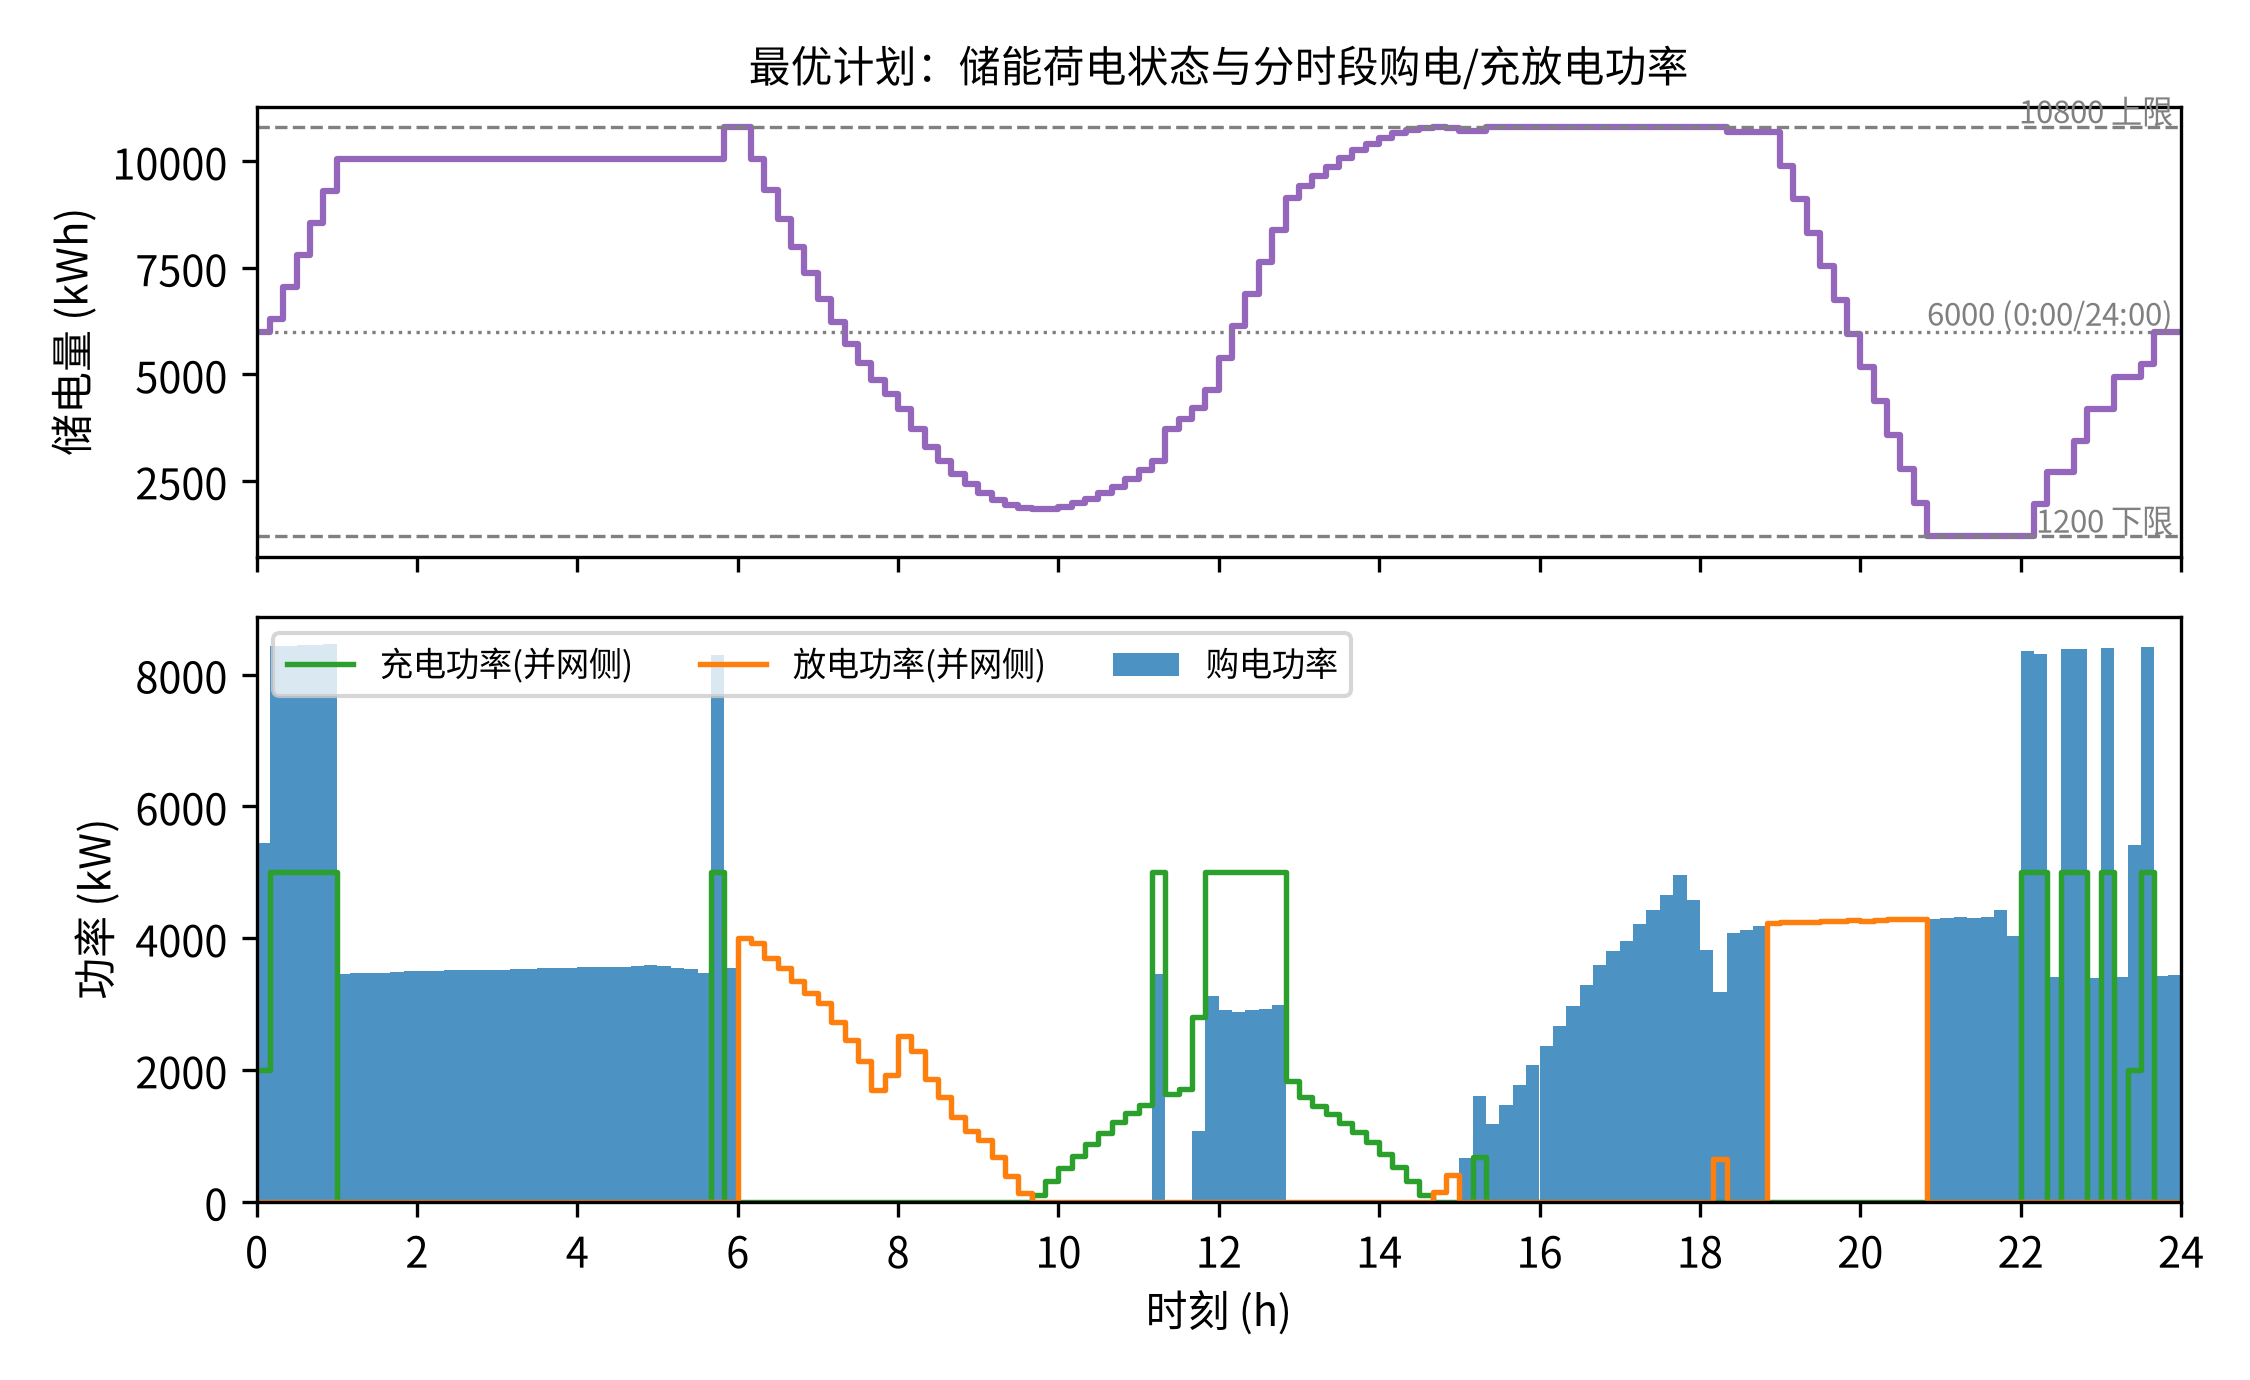
\includegraphics[width=0.72\textwidth]{fig2_dispatch.png}
\caption{最优计划下的储能荷电状态与各时段购电、充电、放电功率}
\label{fig:dispatch}
\end{figure}

\subsection{对偶分析及最优性证明}

LP 的对偶变量给出比数值解更深一层的解释。我们给各类约束挂上影子价格，据此定义节点边际价值 $\gamma_t$：在时段 $t$ 末白得 1~kWh 储能，全天购电费能省下多少。$\gamma$ 沿时间轴满足递推
\begin{equation}
\gamma_t=\gamma_{t+1}-\eta_t+\theta_t ,
\label{eq:gamma}
\end{equation}
其中 $\eta_t$、$\theta_t$ 是储电量上、下限约束的对偶变量。内点节点上 $\gamma$ 逐段不变，能量躺在罐里不生息；满罐节点 $\gamma$ 下移 $\eta_t$，空罐节点 $\gamma$ 上移 $\theta_t$。由 KKT 互补松弛条件可得充放电的三条启停判据，对偶理论见文献~\cite{boyd2004}。充电段满足 $\lambda_t=0.9\gamma_t$，功率顶格段另加正的影子溢价；放电段满足 $\sigma_t=\gamma_t/0.9$，$\sigma_t$ 为该段边际供电成本；空闲段的价格落在 $0.9\gamma_t$ 与 $\gamma_t/0.9$ 之间的迟滞带内。把充、放电段的等式联立，可得跨窗口搬运能量的门槛，放电价与充电价之比须不低于
\begin{equation}
\frac{1}{0.81}\approx 1.235 .
\label{eq:th}
\end{equation}
说白了，价差比不到 1.235 的两段之间，LP 一千瓦时也不会搬。同一段内边充边放要求 $\lambda_t=0.9\gamma_t$ 与 $\lambda_t=\gamma_t/0.9$ 同时成立，推出 $\gamma_t=0$ 且 $\lambda_t=0$；本问电价恒为正，故最优解中不存在同段充放，无需为排除该行为引入 0-1 变量，这与文献~\cite{wangxz2017} 用状态变量处理储能充放互斥的做法形成对照。

图~\ref{fig:shadow} 画出 $\gamma$ 与 $\lambda$ 的全天对比。两处结构最能说明问题。其一，两个放电大窗口 6:00-9:40 与 18:50-20:50 内 $\sigma$ 分别为 0.591 与 1.256 元/kWh，都低于当时的电价，储能把两个价格峰完全削平，窗口内购电为零。其二，15:10-18:30 储电量顶在 10800~kWh 的平台期，$\gamma$ 从 0.733 爬升至 1.130 元/kWh，每经过一个满罐节点上移一点，罐容稀缺的影子价随放电临近在累积。最优性方面，互补松弛条件在全时段的违约不超过 $1.4\times10^{-17}$ 元/kWh，节点价值的有限差分重解与对偶值偏差为 $1.2\times10^{-12}$，两条独立途径相互印证。

\begin{figure}[htbp]
\centering
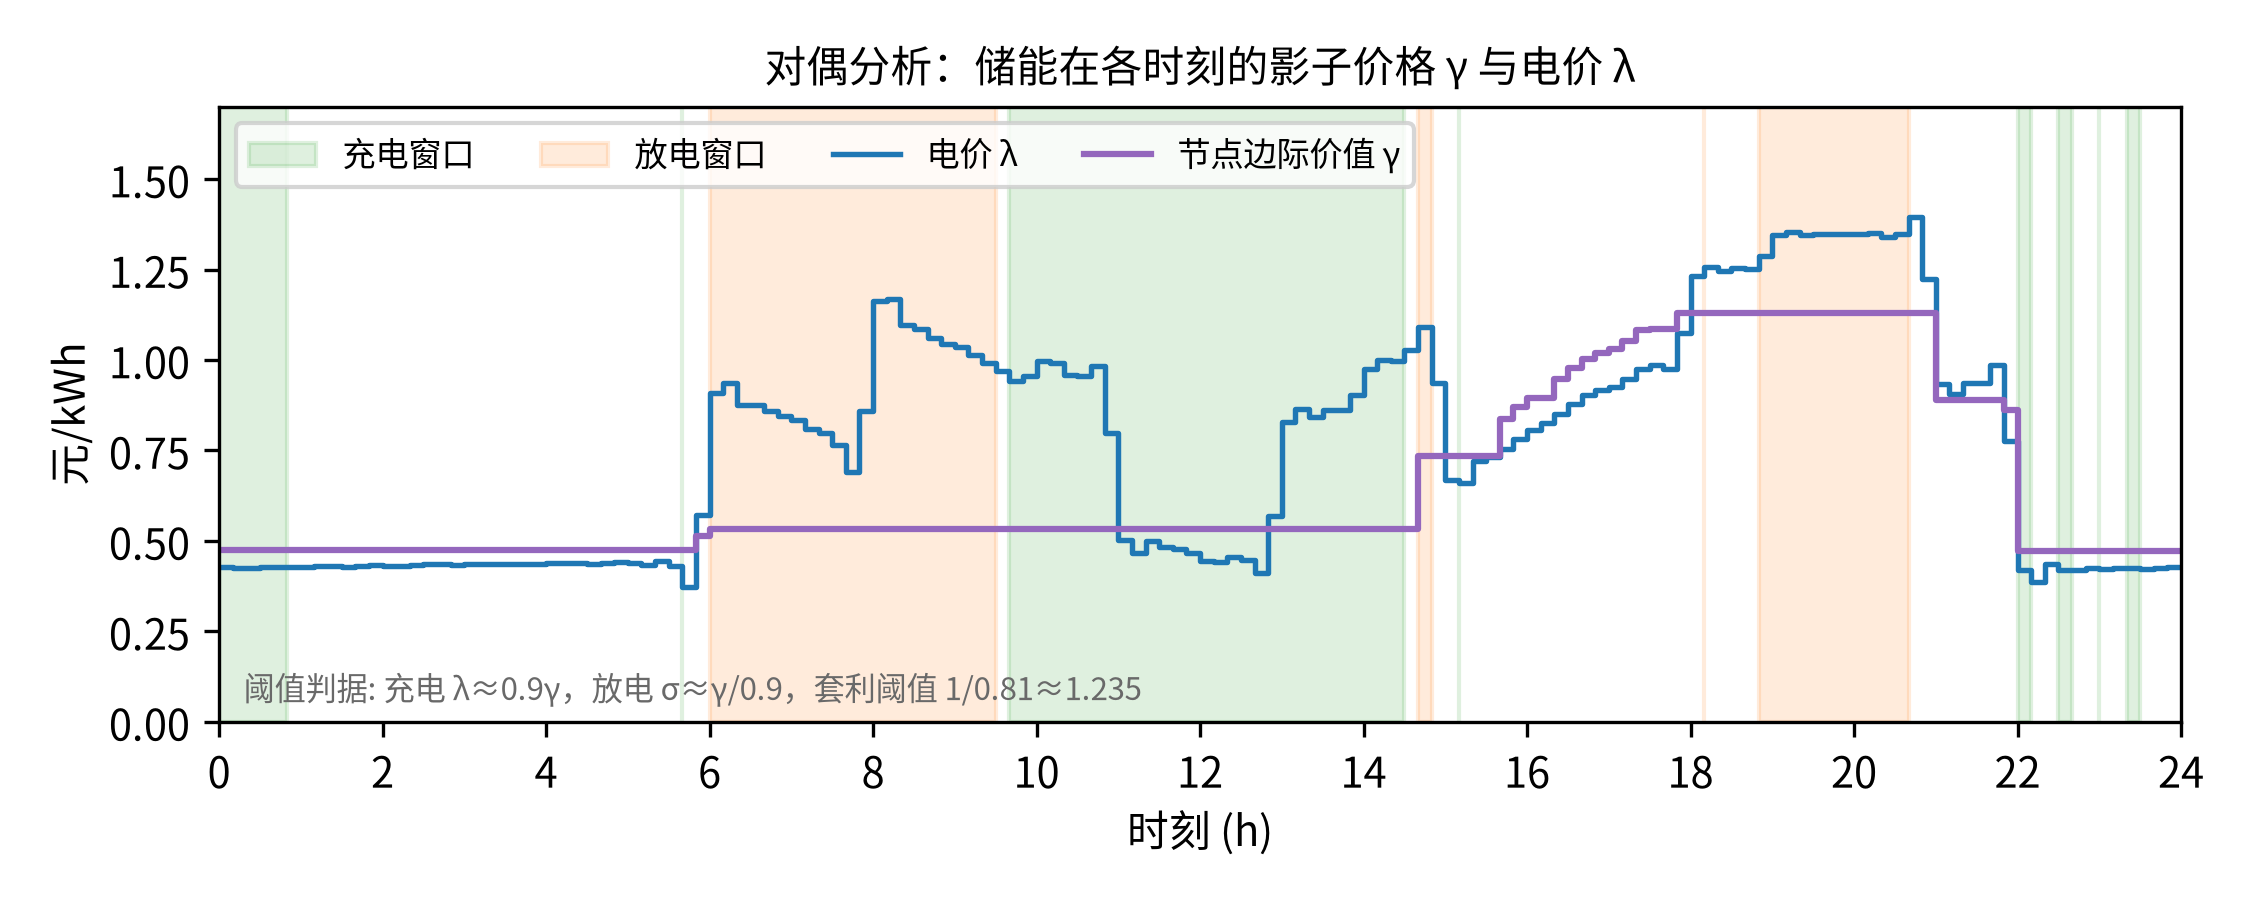
\includegraphics[width=0.72\textwidth]{fig3_shadow.png}
\caption{储能节点边际价值 $\gamma$ 与电价 $\lambda$ 的全天对比，底色标出充放电窗口}
\label{fig:shadow}
\end{figure}

\subsection{模型评价}

灵敏度扫描围绕充放电效率 $\eta$ 展开，取 0.85 至 0.95 共五档做完整重解，用意不在改动题面给定的 90\%，而在展示成本对该参数的响应结构，结果见表~\ref{tab:sens}。成本随 $\eta$ 单调下降，每提高 0.01 约降 0.5\%；失效边界在 $\eta\approx0.84$ 附近，早峰需放电 8068.8~kWh，满罐可放量为 $(10800-1200)\,\eta$，$\eta$ 低于 $8068.8/9600\approx0.841$ 后单个日循环放不满早峰缺口，必须在午间二次回充，成本上升明显加快。功率上限的敏感性小得多，把 $P_{\max}$ 从 5000~kW 放宽到 6000~kW，成本仅降 0.12\%，说明 19 个顶格充电时段并不构成主要瓶颈。

\begin{table}[htbp]
\centering
\caption{充放电效率 $\eta$ 的敏感性扫描}
{\small
\begin{tabular}{cccc}
\toprule
$\eta$ & 阈值 $1/\eta^2$ & 购电费/元 & 较 $\eta=0.90$ \\
\midrule
0.85 & 1.384 & 36603.21 & $+4.20\%$ \\
0.88 & 1.291 & 35696.82 & $+1.62\%$ \\
0.90 & 1.235 & 35126.85 & 题面取值 \\
0.92 & 1.182 & 34575.53 & $-1.57\%$ \\
0.95 & 1.108 & 33767.02 & $-3.87\%$ \\
\bottomrule
\end{tabular}}
\label{tab:sens}
\end{table}

为检验全局优化的价值，我们复现了文献中常见的规则式策略~\cite{wangxz2017,wangly2020}作为对照：光伏先直供、盈余充电；电价低于全日 20\% 分位 0.4333 元/kWh 时电网充电，高于 80\% 分位 1.0060 元/kWh 时放电，其余时段直购；最后按闭环要求修正储电量。该策略全天购电费 39241.62 元，比 LP 最优贵 11.71\%。这个差距不小。追根溯源有两处，其一，分位阈值一刀切，80\% 分位漏掉了早峰 0.69~1.00 元/kWh 的放电机会，这一段只能高价直购；其二，规则不带前瞻，罐体早早充满，全日最低价时段与午后光伏盈余互相挤占容量。LP 把存什么、何时存、何时用做全局配对，两处损失都被消除。

% ===================== 6-8 问题2/3/4（占位） =====================
\section{问题2模型的建立与求解}
% TODO：全年实际数据（附件2），逐日 0:00 只用历史信息预测负载与光伏（见交接文档），
% 以预测值仿照问题1建立计划购电模型；实际缺口按交易时刻电价 5 倍紧急购电；
% 输出 result2.xlsx（计划购电量、充放电量、紧急购电量），2025.2.1 起逐日。

\section{问题3模型的建立与求解}
% TODO：附件3 提供每日 0/6/12/18 点的未来 24 小时光伏预报；0:00 制定计划购电，
% 其他时刻制定调整购电；计划高于调整为违约部分按 0.5 倍价、调整为超购部分按 1.5 倍价；
% 需分析是否值得引入其他时刻的预报；输出 result3.xlsx。

\section{问题4模型的建立与求解}
% TODO：附件4 波动电价替代分时电价，重算问题2与问题3；输出 result4-2.xlsx、result4-3.xlsx。

% ===================== 9 总结（占位） =====================
\section{模型评价与总结}
% TODO：逐条回答四个问题的最终数值结论；优缺点对着模型说并量化（效率口径 ±、
% 完全信息假设的局限）；不复述摘要，不引入新内容。

% ===================== 参考文献 =====================
{\small
\begin{thebibliography}{9}
\bibitem{wangxz2017} 王先齐, 吕智林, 汤泽琦. 基于分时电价机制的并网型微网多目标动态优化调度[J]. 电力系统保护与控制, 2017, 45(4). DOI: 10.7667/PSPC160250.
\bibitem{yuanlong2018} 袁龙. 分布式光伏发电与储能协同调度模型研究[D]. 济南: 山东大学, 2018.
\bibitem{sioshansi2009} Sioshansi R, Denholm P, Jenkin T, et al. Estimating the value of electricity storage in PJM: Arbitrage and some welfare effects[J]. Energy Economics, 2009, 31(2): 269-277.
\bibitem{wangly2020} 王凌云, 王晓敏, 胡兴媛, 等. 基于多智能体微网的需求侧分时电价优化调度[J]. 信息与控制, 2020, 49(4): 429-435.
\bibitem{boyd2004} Boyd S, Vandenberghe L. Convex Optimization[M]. Cambridge: Cambridge University Press, 2004.
\end{thebibliography}
}

% ===================== AI 使用声明（占位） =====================
\section*{AI 工具使用声明}
% TODO（2026 新规）：按竞赛当期规范声明 AI 工具的使用环节与方式，并在支撑材料中附
% 《AI工具使用详情.pdf》（工具版本/目的环节/提示方式/采纳核验情况）。
（占位）本项按竞赛当期规范填写。

\end{document}
